% +--------------------------------------------------------------------+
% | Sample Chapter 3
% +--------------------------------------------------------------------+

\cleardoublepage

% +--------------------------------------------------------------------+
% | Replace "This is Chapter 3" below with the title of your chapter.
% | LaTeX will automatically number the chapters.                      
% +--------------------------------------------------------------------+

\chapter{Model Development}
\label{chp3}

Chapter \ref{chp3} will be dedicated to developing the various parameters that make up the NERMLAB such as the motor torque constant, \ac{back-emf}, inductance, and max voltage. Each section in Chapter \ref{chp3} will detail the process of how the various parameters were measured, calculated, and experimentally determined. Nomenclature for various constants and parameters are detailed in the table \ref{table2}.

% Table of motor lab constants
\begin{table}[ht]
\begin{center}
\caption{Motor parameters}
\begin{tabular}[c]{|c|c|}

\hline
\textbf{Parameter} & \textbf{Description}\\

\hline
V & Motor Voltage\\

\hline
\(k_t\) & Motor Torque Constant per Phase\\

\hline
\(k_T\) & Overall Motor Torque Constant\\

\hline
\(K_e\) & Back Electromotive Force Constant per Phase\\

\hline
\(K_{e,LL}\) & Line-Line Back Electromotive Force Constant\\

\hline
J & Mass Moment of Inertia\\

\hline
L & Motor Inductance\\

\hline
R & Motor Resistance\\

\hline
\(\tau\) & Time Constant\\

\hline
T & Motor Torque\\

\hline
\end{tabular}

\label{table2}
\end{center}
\end{table}

% end of table

\section{Motor Resistance}

\section{Motor Torque Constant and Back EMF}
The motor torque constant (\(k_t\)) is a common parameter used in BLDC motors. It relates the armature current to the torque produced by a motor: \(T = k_T i \). Many methods exist to determine the torque constant, including relating the motor velocity constant \(k_v\) which is inversely related to the torque constant by \(k_T = \frac{1}{k_v} \), or by measuring the line-line back-emf voltage per phase (\(K_e\)). \(K_e\) is the peak value of the back-emf per angular velocity measured from line-neutral. However since line-neutral is typically unavailable on most BLDC motors, the back-emf constant is often represented as a line measurement, \(K_{e,LL}\). The overall torque constant can then be related to the line measurement back-emf for sinusoidal type outputs by equation | \citep{5}. 

\[k_T = \frac{\sqrt{3}}{2} K_{e,LL}\]

Because \(K_{e,LL}\) can be experimentally determined, it is possible to find the overall motor torque constant for a BLDC motor. One simply needs to measure the line-line sinusoidal\footnote{Note in the case of trapezoidal waveforms the relationship between \(k_T\) and \(K_{e,LL}\) are proportional, i.e. \(k_T = K_{e,LL}\)} back-emf voltage at various speeds to get a good estimate of \(K_{e,LL}\), then in conjunction with equation | \(k_T\) can then be determined.

\subsection{Procedure}
Outline of the experimental procedure done to measure Kt.

\[K_E = \frac{V}{\omega_m}\]

\section{Mass Moment of Inertia Estimation}
Mass moment of inertia \(J\) is the equivalent to mass in a rotational system (commonly referred to as angular mass). More formally is it defined as \(J = \int r^2 dm\), where r is the distance to some mass from an axis of rotation.

The angular mass of the NERMLAB will be determined in two ways: experimentally determining \(J\) through software modeling, and approximating \(J\) through mathematical formulation. For both setups the mass of the rotating inertia had to be measured.

\subsection{Software Modeling of Mass Moment of Inertia}
\subsection{Mathematical Approximation of Mass Moment of Inertia}
To simplify the mathematical analysis of the mass moment of inertia calculation of the angular mass of the NERMLAB, an engineering assumption will be made that the angular mass is a rotating ring mass. This assumption is valid for the particular motor used in this thesis due to the fact that most of the mass is concentrated around the outside parameter of the motor. The outside ring mass of the motor contributes the most to the inertial load, so the mathematical formulation would result in the following equation:
\[J_z = \frac{m}{2}(r_1^2 + r_2^2) = mr_2^2(1-t+\frac{t^2}{2})\]

\begin{figure}[htb]%t=top, b=bottom, h=here
\begin{center}
    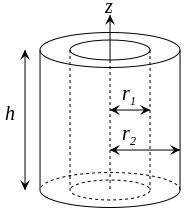
\includegraphics[height=1.5in]{figures/thick_walled_cylinder.png}

    \caption[Thick Walled Cylinder - Mass Moment of Inertia]{Thick Walled Cylinder (J)}

    \label{thick_walled_cylinder}
\end{center}
\end{figure}

\section{Motor Inductance}

\[L = R\tau\]